\documentclass[notes]{subfiles}
\begin{document}
	\addcontentsline{toc}{section}{1.9 - Quadratic Functions \& Models}
	\refstepcounter{section}
	\fancyhead[RO,LE]{\bfseries  \large \nameref{cs19}} 
	\fancyhead[LO,RE]{\bfseries \currentname}
	\fancyfoot[C]{{}}
	\fancyfoot[RO,LE]{\large \thepage}	%Footer on Right \thepage is pagenumber
	\fancyfoot[LO,RE]{\large Chapter 1.9}


\section*{Quadratic Functions \& Models}\label{cs19}
	\subsection*{Quadratic Models}
		The model is given by $f(x) = ax^2 + bx + c$, where $a,b,c$ are constants ($a\neq 0$).  The function has an absolute maximum if $a < 0$, and absolute minimum if $a > 0$.
		\begin{figure}[h!]
		\fbox{
		\begin{minipage}{1in}
			\centering
			$\underline{a > 0}$\\
				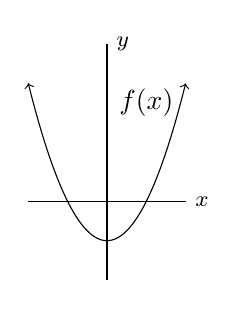
\begin{tikzpicture}[x = .5cm, y = .5cm]
					\draw (-2,0)--(2,0) node[right] {\footnotesize $x$}; %x-axis 
					\draw (0,-2)--(0,4) node[right] {\footnotesize $y$}; %y-axis
					\draw[<->, smooth, samples = 100, domain = -2.:2.] plot (\x, {(\x)^2 - 1});	
					\draw (1,2.5) node {$f(x)$};
				\end{tikzpicture}	
		\end{minipage}
		\begin{minipage}{2in}
			\begin{itemize}
				\item $\ds \lim_{x\to\infty} f(x) =$ \showto{ins}{\fbox{$\infty$}}\showto{st}{}
				\item $\ds \lim_{x\to -\infty} f(x) =$ \showto{ins}{\fbox{$\infty$}}\showto{st}{}
				\item $f$ is decreasing then increasing
				\item $f$ is concave up 
			\end{itemize}
		\end{minipage}
		}
		\fbox{
		\begin{minipage}{1in}
			\centering
			$\underline{a < 0}$\\
				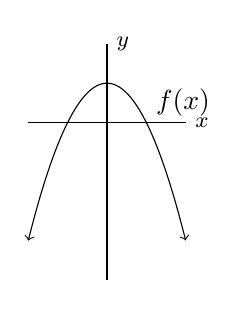
\begin{tikzpicture}[x = .5cm, y = .5cm]
					\draw (-2,0)--(2,0) node[right] {\footnotesize $x$}; %x-axis 
					\draw (0,-4)--(0,2) node[right] {\footnotesize $y$}; %y-axis
					\draw[<->, smooth, samples = 100, domain = -2.:2.] plot (\x, {-(\x)^2 + 1});	
					\draw (1,.5) node[right] {$f(x)$};
				\end{tikzpicture}
		\end{minipage}
		\begin{minipage}{2in}
			\begin{itemize}
				\item $\ds \lim_{x\to\infty} f(x) =$ \showto{ins}{\fbox{$-\infty$}}\showto{st}{}
				\item $\ds \lim_{x\to -\infty} f(x) =$ \showto{ins}{\fbox{$-\infty$}}\showto{st}{}
				\item $f$ is increasing then decreasing
				\item $f$ is concave up then down
			\end{itemize}
		\end{minipage}
		}
		\end{figure} 
			
	\subsection*{Choosing Models}
		At this point, we have five models to choose from when analyzing a data set.  The process of choosing a model should go as follows:
		\begin{itemize}
			\item Does the scatterplot show any sort of concavity?  If yes, then go to the next step.  If not, try a \textbf{linear} model.
			\item If the scatterplot shows concavity, does it appear to \emph{change concavity}? If yes, then the model could be \textbf{logistic} or \textbf{cubic}.  If not, then the model could be \textbf{exponential}, \textbf{logarithmic}, or \textbf{quadratic}.
			\begin{enumerate}
				\item If the scatterplot changes concavity, then does it have an asymptote? If yes, then the model is \textbf{logistic}.  If no, then the model is \textbf{cubic}.
				\item If the scatterplot does not change concavity, then look at the end behavior and for asymptotes.  If there is an asymptote at $x = 0$, then the model is \textbf{logarithmic}; if it is at $y = 0$, then the model is \textbf{exponential}; if there is no asymptote, then it is \textbf{quadratic}.
			\end{enumerate}
		\item If it is still difficult to determine between exponential and quadratic, then use the method of second differences (described below).  If second differences gives roughly constant values, then the model is \textbf{quadratic}; if it does not, then, it is \textbf{exponential}.
		\item If in doubt, one can develop multiple models and compare the fit of each model against the data.
		\item It is never a bad idea to apply common sense to models.
		\end{itemize}
			\newpage
		\begin{ex}
			Draw a decision tree/diagram for choosing a model.
			\vs{3}
		\end{ex}
		
		\begin{ex}
			The table below shows the profit (in millions of dollars) that American Airlines makes on tickets between Dallas and Chicago when tickets are set at a certain price:
				\begin{center}
					{\renewcommand{\arraystretch}{1.2}
					\begin{tabular}{|c||c|c|c|c|c|c|}\hline
						\textbf{Ticket Price} (dollars) & 200 & 250 & 300 & 350 & 400 & 450 \\ \hline
						\textbf{Profit} (million dollars) & 3.08 & 3.52 & 3.76 & 3.82 & 3.7 & 3.38\\ \hline
					\end{tabular}
					}
				\end{center}
				\begin{enumerate}[(a)]
					\item Give two reasons why a quadratic model is more appropriate than a log or exponential model.
						\vs{1}
					\item Find a quadratic model for the data.
						\vs{1}
						\newpage

					\item Why doesn't the airline profit increase as the ticket price increases?
						\vs{.5}
					\item At what price does the airline begin posting a loss?
						\vs{.5}
				\end{enumerate}
		\end{ex}
		
		\begin{ex}
			The table below gives the braking distance required for a vehicle to come to a complete stop, given the initial velocity of the vehicle.
				\begin{center}
					{\renewcommand{\arraystretch}{1.2}
					\begin{tabular}{|c||c|c|c|c|c|c|c|c|c|}\hline
						\textbf{Speed} (mph) & 10 & 20 & 30 & 40 & 50 & 60 & 70 & 80 & 90 \\ \hline
						\textbf{Distance} (feet) & 27 & 63 & 109 & 164 & 229 & 304 & 388 & 481 & 584\\ \hline
					\end{tabular}
					}
				\end{center}
				\begin{enumerate}[(a)]
					\item Find the second differences of the data above.
						\vs{1.5}
					\item Find a quadratic model for stopping distance.
						\vs{1}
					\item What other factors besides the initial speed would impact the stopping distance?
						\vs{.5}
					\item What speed is the vehicle moving if its braking distance is exactly 412 feet?  Round your answer to two decimal places, if needed.
						\vs{.5}
				\end{enumerate}
		\end{ex}
			\newpage

		\begin{ex}
			The ratios of public school students to instructional computers with Internet access for years between 1998 and 2004 are given below:
				\begin{center}
					{\renewcommand{\arraystretch}{1.2}
					\begin{tabular}{|c||c|c|c|c|c|c|c|}\hline
						\textbf{Year} & 1998 & 1999 & 2000 & 2001 & 2002 & 2003 & 2004 \\ \hline
						\textbf{Ratio} & 9.1 & 6.1 & 3.6 & 2.4 & 1.8 & 1.4 & 1.8\\ \hline
					\end{tabular}
					}
				\end{center}
				\begin{enumerate}[(a)]
					\item Align the input so that 1998 corresponds to an input of 0.
					\item Write the complete quadratic model for the data.
						\vs{1}
					\item Write the complete exponential model for the data.
						\vs{1}
					\item Which model best fits the data: (b) or (c)?
						\vs{.5}
					\item Give two reasons why an exponential model might be best for this data.
						\vs{1}
				\end{enumerate}
		\end{ex}

	
	\clearpage
\end{document}